\chapter{Concepte Teoretice}

\section{Rețele neuronale}

Rețelele neuronale stau la baza tuturor algoritmilor moderni de inteligență artificială. Acestea au revoluționat industria învățării automate prin puterea lor de a simula funcțiile cognitive ale creierului uman, fiind des folosite in invățarea de tipare(în engleză pattern recognition), diferite sarcini de clasificare si predicție. Ele pot fi văzute ca funcții complicate care primesc date de intrare sub forma unor valori numerice și returnează valori reprezentative pentru acestea. 

\subsection{O scurtă istorie a rețelelor neuronale}

\begin{itemize}
    \item În lucrarea intitulată „A Logical Calculus of the Ideas Immanent in Nervous Activity”(1943) \cite{mcculloch1943logical} Warren McCulloch și Walter Pitts au fost primii care au teoretizat o implementare matematică simplificată a neuronului ca o poartă logică binară. Aceștia au demonstrat teoretic faptul că neuronii au capacitatea de a reprezenta orice funcție matematică.

    \item În 1958, este publicată lucrarea cercetătorului Frank Rosenblatt „The Perceptron: A Probabilistic Model for Information Storage and Organization in the Brain” \cite{rosenblatt1958perceptron}, în care acesta introduce conceptul de Perceptron, cel mai simplu model de rețea neuronală. 

    \newpage
    
    \item Spre finalul anilor 1980, după o lungă perioadă în care studiul rețelelor neuronale a fost neglijat, David E. Rumelhart, Geoffrey Hinton, and Ronald J. Williams (1986) \cite{rumelhart1986learning} prezintă \textbf{backpropagarea}, un algoritm prin care o rețea neuronală putea să învețe eficient, adresând multe dintre problemele ridicate până la acel moment. 

    \item La începutul anilor 2000, tot Geoffrey Hinton, de data aceasta alături de Ruslan Salakhutdinov \cite{hinton2006reducing} aduc o soluție pentru problema gradienților care dispar, prin reducerea dimensionalității datelor.
\end{itemize}

Aceste lucrări din literatură au ajutat la transformarea unor concepte pur teoretice în unelte cu putere de învățare și de decizie care au ajutat la modelarea industriei moderne și au împins progresul tehnologic către noi limite. 

\subsection{De la neuronul biologic la cel artificial}
    La fel ca multe dintre invențiile revoluționare de-alungul istoriei, cercetătorii au avut ca sursă de insipirație viețuitoarele. În cazul inteligenței artificiale, aspirația cercetătorilor a fost să replice neuronul biologic. 
    
    \begin{figure}[h]
         \centering 
         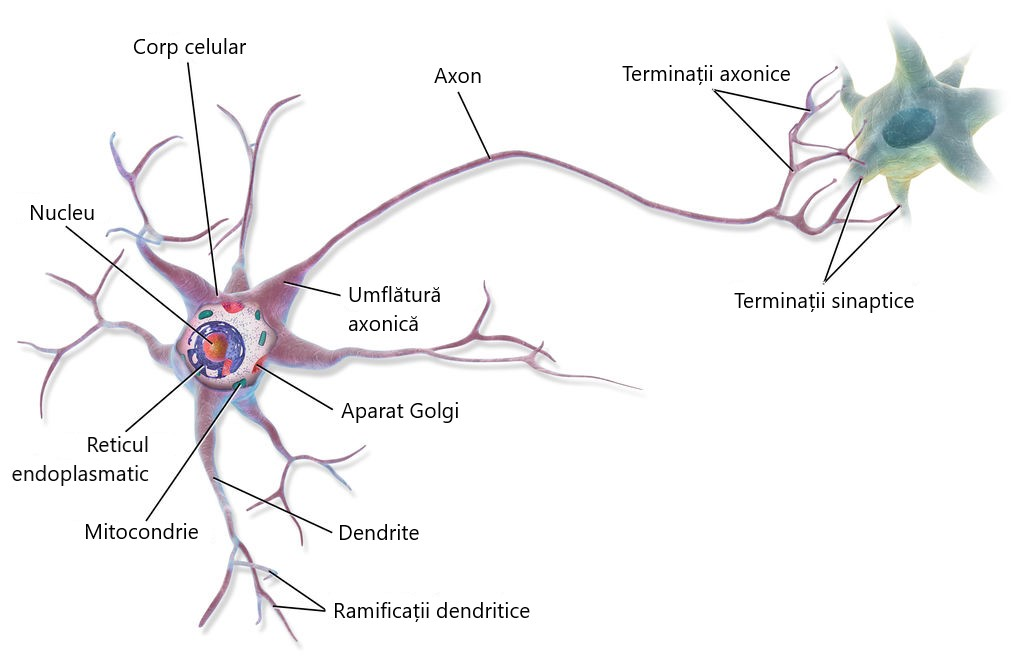
\includegraphics[width=.75\textwidth]{images/structura-unui-neuron.jpg}
         \caption{Anatomia unui neuron \cite{neuron-anatomy}}
    \end{figure}
    
    În zona centrală a neuronului se află corpul celular(soma) care conține nucleul, locul care înmagazineaza tot materialul genetic al celulei. Legate de corpul celular sunt dendritele, care interceptează semnale chimice de la alți neuroni. Atașat de corpul celular, se află o prelungire alungită numită axon, al cărei scop este să transmită semnale electrice către alți neuroni sau către țesuturi. La capătul axonului se găsesc terminațiile acestuia, care sunt legate de dendritele sau de corpul celular ale altui neuron. 

    În creierul biologic, se găsesc miliarde de neuroni, fiecare având mii de legaturi cu alți neuroni aceștia fiind dipusi in straturi pentru a crea țestul nervos. Cu toate că neuronul in sine, nu funcționează intr-un mod complex, ansamblul a miliarde de mecanisme simple într-o rețea imensa are capabilități impresionante. 

    Plecând de la aceste premise Warren McCulloch și Walter Pitts(1943) 
    \cite{mcculloch1943logical} au prezentat în lucrarea lor revoluționară o versiune simplificată a neuronului biologic. Aceștia au văzut neuronul artificial ca o pe poartă logică, cu mai multe intrări și o singură ieșire. Un semnal electric era transmis mai departe doar dacă neuronul avea un număr de intrări care trecea de un anumit prag, bazându-se pe principiul de totul sau nimic al neuronilor biologici.  

     \begin{figure}[h]
         \centering 
         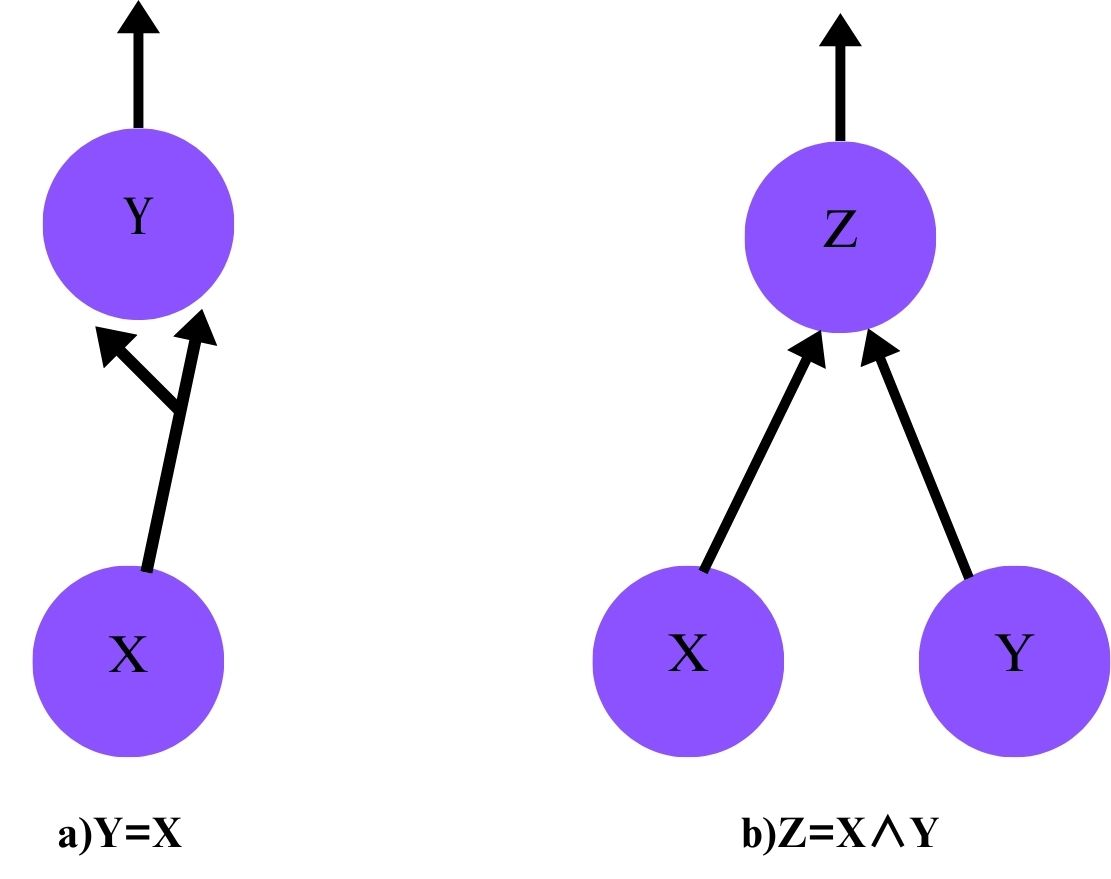
\includegraphics[width=.5\textwidth]{images/artificial-neurons-as-logic-gates.jpg}
         \captionsetup{font=footnotesize}
         \caption{Neuroni artificiali calculând operatii logice}
         \caption*{a) Neuronul Y nu poate transmite semnalul mai departe              doar cu un singur impuls}
         \caption*{b) Neuronul Z are nevoie de ambii neuroni X și Y pentru a trimite un semnal mai departe}
    \end{figure}

    \newpage

\subsection{Perceptronul}

În 1958 Frank Rosenblatt \cite{rosenblatt1958perceptron} introduce in literatură \textbf{perceptronul}, cel mai simplu model de rețea neuronală. Acesta duce neuronul artificial propus de către McCulloch și Pitts \cite{mcculloch1943logical} la un alt nivel. Comparat cu neuronul care transmitea doar semnale binare, cel propus de Rosenblatt este capabil sa proceseze și să transmită mai departe valori numerice. Scopul final este de a organiza aceste unități de calcul într-o „rețea” care primește datele de intrare sub formă numerică și returnează o valoare care le reprezintă. 

Într-o astfel de rețea fiecare neuron se folosește datele de intrare pentru a produce o valoare de ieșire. Fiecărei valori de intrare îi corespunde o pondere(în engleză: weight), un număr real al cărui scop este sa controleze contribuția sa la informația transmisă mai departe de către neuron. Aceste valori sunt însumate ponderat, iar la valoarea obținută se adaugă un neuron special, care la rândul lui are o pondere. Acest neuron se numește \textit{bias}, un număr real, notat cu $b$, care elimină constângerea ca funcția ce reprezintă datele să treacă prin originea planului sau a hiperplanului. Rezultatul reprezintă o funcție care este dată ca parametru unei funcții liniare numită „funcție de pas”(in engleză: step function) pentru a produce valoarea de ieșire a perceptronului. 

\begin{figure}[h]
         \centering 
         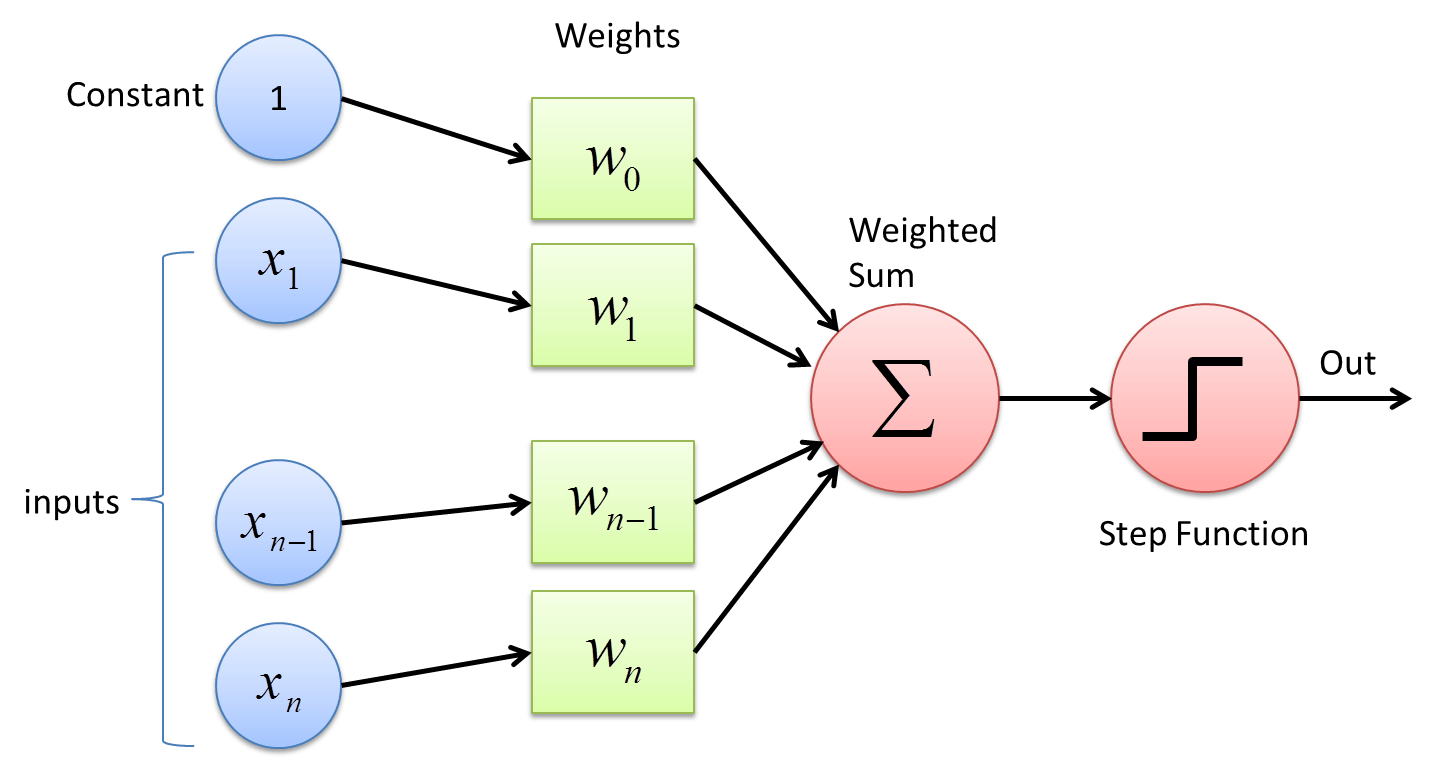
\includegraphics[width=.85\textwidth]{images/the-perceptron.jpg}
         \captionsetup{font=footnotesize}
         \caption{Perceptronul \cite{the-perecptron}}
\end{figure}
\newpage
Notații:

\begin{itemize}
    \item $x = (x_1, x_2, x_3... , x_n)$ datele de intrare
    \item $w = (w_1, w_2, w_3,..., w_n)$ ponderile corespunzătoare 
    \item $b$ = totalitatea neuronilor de \textit{bias} 
    \item $z$ = combinația liniară dintre $x$ si $w$
    \item $z = w_1 x_1 + w_2 x_2 + ... + w_n x_n  = \sum_{i=1}^{n} w_i x_i + b = w^{T}x + b$
    \item $step(z)$ = \textit{output-ul} perceptronului
\end{itemize}
 
O funcție comună folosită drept \textit{step function} este funcția semn definită astfel: 

\[
\text{sgn}(x) = 
\begin{cases} 
    -1 & \text{if } x < 0, \\
    0 & \text{if } x = 0, \\
    1 & \text{if } x > 0.
\end{cases}
\]    

\begin{figure}[h]
         \centering 
         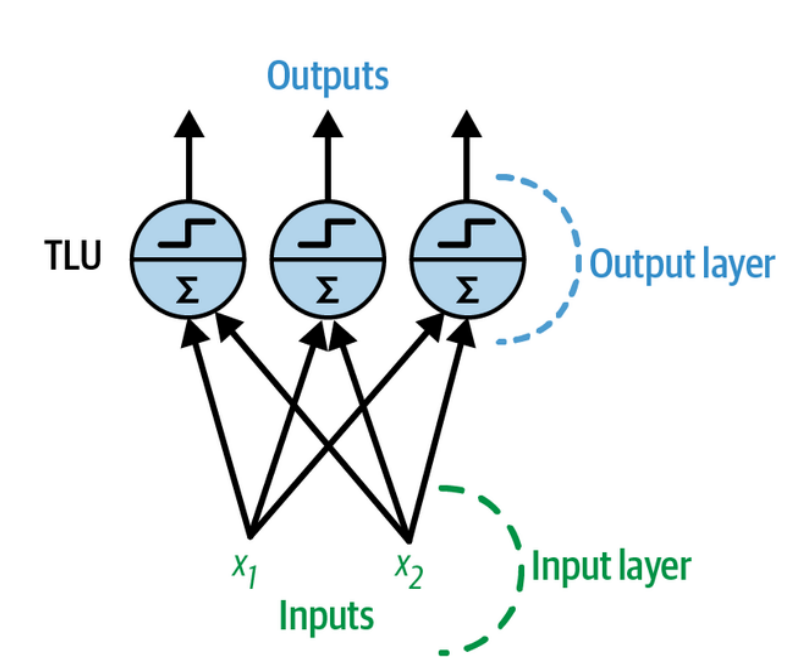
\includegraphics[width=.5\linewidth]{images/multiclass-perceptron.png}
         \captionsetup{font=footnotesize}
         \caption{Un perceptron capabil să separe date în mai multe clase \cite{ageron2019}}
         \label{Figura 2.4}
\end{figure}
\newpage

În Figura~\ref{Figura 2.4} este prezentată o arhitectură de perceptron capabilă sa distingă între 3 clase. Datele de intrare, in cazul nostru $x1$, $x2$ reprezintă \textit{stratul de intrare}. Fiecare valoare din stratul de intrare este legată de toți neuronii din stratul urmator, fiecare legatură având o pondere individuală. Stratul care produce valorile de ieșire se numește \textit{stratul de ieșire} și in exemplul prezentat este format din 3 neuroni, corespunzători fiecărei clasificări posibile. 

În ciuda optimismului declanșat de capabilitățile remarcabile la acea vreme a perceptronului, în 1969 Marvin Minsky și Seymour Papert \cite{minsky1969introduction} au demonstrat limitarea acestui model de a rezolva cateva probleme triviale, precum operația XOR. 

\subsection{Multilayer Perceptron(MLP)}

Soluția pentru limitările perceptronului a fost unificarea mai multor rețele de tip perceptron intr-o rețea mai mare, numita Multilayer Perceptron(MLP). Noua clasificare a straturilor este :

\begin{itemize}
    \item Stratul de input = stratul ce conține doar valorile de intrare
    \item Straturile ascunse = straturile prin care se propaga informația. Se sitează între stratul de input și cel de output
    \item Stratul de output = stratul care ne oferă rezultatul trecerii informației prin rețea
\end{itemize}

% \newpage

\begin{figure}[h]
         \centering 
         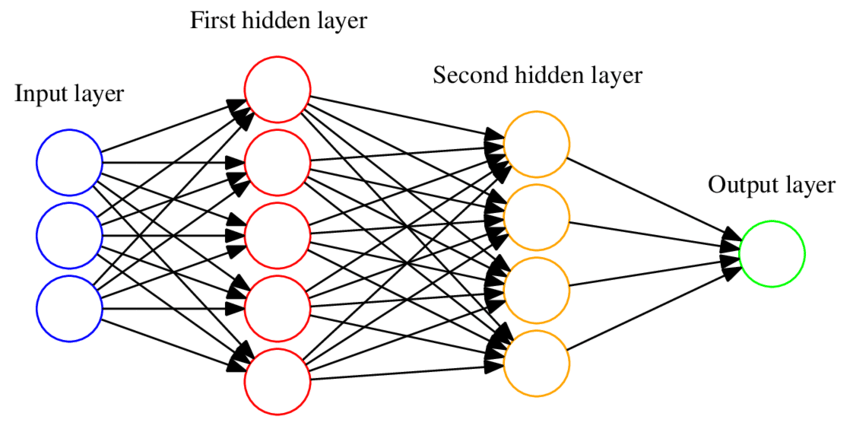
\includegraphics[width=.6\linewidth]{images/MLP.png}
         \captionsetup{font=footnotesize}
         \caption{Arhitectura de tip MLP(Multilayer Perceptron) \cite{phdthesis}}
\end{figure}
    
Arhitectura MLP este una de tip \textbf{feedforward}, cu alte cuvinte, informația se propagă prin rețea intr-o singură direcție, de la stânga la dreapta(dinspre input către output).

\subsection{Backpropagarea}

Algoritmul prin care o rețea neuronală învață se numește \textbf{backpropagation}. Acesta presupune trecerea prin rețea în repetate rânduri, în doi pași: unul inainte și unul înapoi. Dupa fiecare trecere parametrii(ponderile) sunt actualizați pentru a obține predicții mai bune.
Algoritmul poate fi descris astfel:
\begin{itemize}
    \item Setul de date este spart în blocuri mai mici, cele mai întâlnite dimensiuni fiind de 32, 64 sau 128 de instanțe per bloc
    \item Fiecare bloc este trecut prin rețea: se calculează output-ul primului strat, care este dat ca intrare pentru urmatorul strat, continuând în același fel până se ajunge la stratul de output. Acesta este pasul forward(\textit{forward pass}).
    \item Se evaluează performanța predicțiilor cu ajutorul unei funcții numită \textbf{funcție de pierdere}. Scopul acestei funcții este să furnizeze un scor care să descrie cât de precise au fost predicțiile rețelei față de rezultatul dorit. 
    \item Dupa calculul erorii, algoritmul calculează contribuția fiecărei ponderi din rețea la eroarea totală, cu ajutorul regulii fundamentale din analiza matematică: regula înlănțuirii(în engleză: \textit{chain rule}).
    \item Contribuția la eroarea totală a unui parametru se numește \textbf{gradient}.Valoarea gradientului practic măsoară cât de mult influențează eroarea totală modificarea acelui parmetru.
    \item În cele din urmă, algoritmul folosește gradienții calculați pentru optimizarea parametrilor cu ajutorul unui algoritm de optimizare.
\end{itemize}
\newpage
\subsection{Algoritmul coborârii pe gradient(\textit{Gradient Descent})}

Coborârea pe gradient este un algoritm iterativ de optimizare, folosit des în literatură, al cărui scop este de găsi minimul global al unei funcții. În cadrul rețelelor neuronale acesta este folosit pentru a optimiza parametrii rețelei astfel încat valoarea erorii totale să se apropie la fiecare iterație de minimul funcției de pierdere. Dupa calcularea gradienților, fiecare pondere se actualizeaza după formula: 
\[
    \scalebox{1.3}{$w_{\text new} = w - \eta \frac{\delta L}{\delta w}$}
\]

Unde: 

\begin{itemize}
    \item $w_{\text new}$ = noua valoare a ponderii
    \item $\frac{\delta L}{\delta w}$ = gradientul 
    \item $\eta$ = rata de învățare(hiperparametru ce controleaza cât de mult se modifică valorile ponderilor)
\end{itemize}

\begin{figure}[h]
         \centering 
         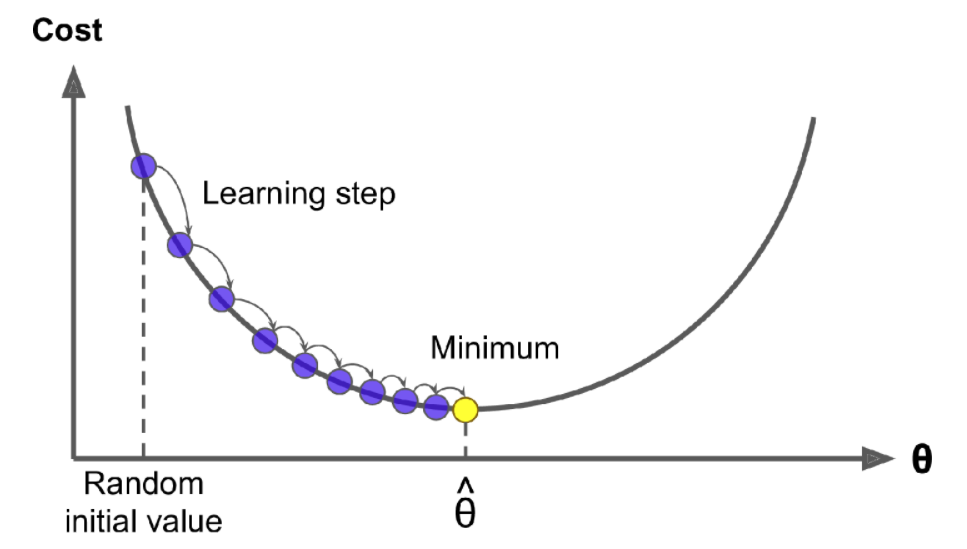
\includegraphics[width=.75\linewidth]{images/gradient-descent.png}
         \captionsetup{font=footnotesize}
         \caption{Vizualizare a algoritmului de coborârii pe gradient \cite{GD}}
\end{figure}

    

